\documentclass[11pt]{article}

% ── Packages ──────────────────────────────────────────────────────────────────
\usepackage[margin=1in]{geometry}
\usepackage{graphicx}
\usepackage{booktabs}
\usepackage{amsmath}
\usepackage{amssymb}
\usepackage{hyperref}
\usepackage{xcolor}
\usepackage{microtype}
\usepackage[numbers,sort&compress]{natbib}
\renewcommand{\bibfont}{\footnotesize}
\setlength{\bibsep}{0pt plus 0.5pt}
\usepackage{subcaption}
\usepackage{multicol}

\hypersetup{
  colorlinks=true,
  linkcolor=blue!60!black,
  citecolor=blue!60!black,
  urlcolor=blue!60!black,
}

\graphicspath{{figures/}}

% Let tall figures share a page with text instead of taking a float page.
\renewcommand{\topfraction}{0.85}
\renewcommand{\bottomfraction}{0.6}
\renewcommand{\textfraction}{0.1}
\renewcommand{\floatpagefraction}{0.8}

% ── Title ─────────────────────────────────────────────────────────────────────
\title{Noesis: Selective Memory Injection for\\Cross-Tool AI Conversation Consistency}

\author{Peizheng Du\\
  Independent Researcher\\
  \texttt{peterdu0628@gmail.com}}
\date{October 2026}

\begin{document}
\maketitle

% ══════════════════════════════════════════════════════════════════════════════
\begin{abstract}
Users converse with several AI assistants, yet each tool's
memory is isolated. Shared and evolving memory layers already exist; this
paper studies a narrower design choice: an explicit rule that decides whether
a captured statement is firm enough to enter the prompt. \textbf{Noesis} is a
local-first memory layer that extracts typed \emph{thoughts} from
conversations across tools into a shared per-user store, injects a thought
only after a confidence lifecycle (repetition, assertion strength, cross-tool
corroboration, no contradiction) promotes it from \emph{tentative}, and caps
injected context with a token budget. On 110 paired synthetic personal
questions, memory injection raises the keyword-hit rate of Gemini Flash-Lite,
gemma3:4b, and qwen2.5:3b by 43.6, 48.2, and 25.5 percentage points (all
$p<0.001$, McNemar's test). At 500 stored memories Noesis injects about 207
tokens, 35 times fewer than injecting everything, with 9 of 10 targets at rank
1; a standard top-5 RAG ranks as well with fewer tokens, so Noesis's distinct
gain is filtering: in two constructed tests, ungated retrieval surfaced
tentative or hedged statements 19 and 13 times, and Noesis surfaced none. Its
gate judges how firmly something was said, not whether it is true. On strictly
cross-tool queries Noesis retrieves 37\% of targets, where per-tool isolation
is bound to 0\%. The code, experiment harness, and raw results are released.

\smallskip\noindent\textbf{Keywords:} large language models; LLM memory;
retrieval-augmented generation; personalization; cross-tool memory;
confidence gating; local-first software
\end{abstract}

% ══════════════════════════════════════════════════════════════════════════════
\section{Introduction}
\label{sec:intro}

Heavy users of AI assistants switch between ChatGPT, Claude, Gemini, and local
models, and each tool keeps its own memory: a preference explained to Claude
must be re-explained to GPT, and the positions and open questions a user works
out in one tool are lost at every tool boundary.

Two families of systems address parts of this problem. \emph{Memory layers}
such as Mem0~\citep{mem0} extract and consolidate facts; OpenMemory
MCP~\citep{openmemory} shares one local store across MCP clients;
Zep~\citep{zep} and Hindsight~\citep{hindsight} track how facts change and how
firmly opinions are held (\S\ref{sec:related}). \emph{Retrieval-augmented
generation} (RAG)~\citep{lewis2020rag} retrieves context per query, but naive
variants inject everything retrieved, so cost grows with memory size and the
relevant signal is buried (I measure 7{,}192 tokens at $n{=}500$).

Noesis is built on a different premise: \emph{what} gets injected matters as
much as \emph{whether} anything is injected. Thoughts should earn their way
into the context the way beliefs earn their way into a mind: through
repetition, consistency, and survival against contradiction. Earning here
means passing an admission rule, not being verified as true.

This paper makes the following contributions:

\begin{enumerate}
  \item \textbf{A confidence lifecycle for conversational memory}
  (\S\ref{sec:system}). Thoughts of seven types mature
  tentative$\to$\allowbreak provisional$\to$\allowbreak settled via a four-signal scorer, with type-specific decay and supersession that cut
  stale-stance leakage from 93\% to 7\% (\S\ref{sec:supersession}).
  \item \textbf{Gated injection that scales}
  (\S\ref{sec:ablation}--\S\ref{sec:scale}). At 500 memories Noesis injects
  $\sim$207 tokens (35 times fewer than injecting everything) at MRR 0.90; top-5 RAG matches that ranking more cheaply, but only Noesis's
  gate keeps tentative and hedged statements out (0 vs.\ 19
  and 0 vs.\ 13 in constructed tests).
  \item \textbf{Quantified cross-tool memory sharing} (\S\ref{sec:crosstool}).
  A shared per-user store retrieves 37\% of strictly cross-tool targets, where
  per-tool isolation scores 0\% by construction (50\% vs.\ 7.5\% over all 40
  scenarios).
  \item \textbf{An A/B result across three model tiers}
  (\S\ref{sec:ab}). On identical $n{=}110$ question sets, memory injection
  significantly raises the keyword-hit rate for a cloud model (Gemini
  Flash-Lite, $+43.6$pp), a mid-tier local model (gemma3:4b, $+48.2$pp), and
  a small local model (qwen2.5:3b, $+25.5$pp); all $p<0.001$.
\end{enumerate}

The system is local-first: embeddings and retrieval run on-device (sqlite-vec
+ all-MiniLM-L6-v2), and conversation text leaves the machine only for
optional cloud extraction or when the proxy forwards a request, with its
injected memories, to a cloud model. Code, experiment harness, saved raw
results, and a script that recomputes every reported number are
released.\footnote{\url{https://github.com/AngryKiwiWithLegs/Noesis}}

\begin{figure}[!htbp]
  \centering
  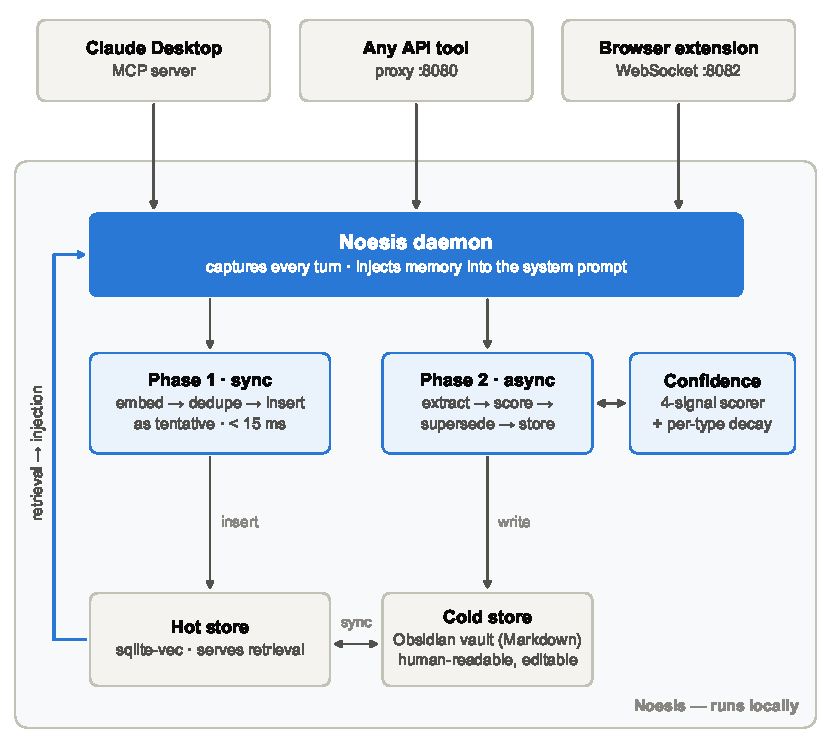
\includegraphics[width=0.64\linewidth]{fig1_architecture.pdf}
  \caption{Noesis architecture. Tools connect through an MCP server, an OpenAI-compatible
  proxy, or a WebSocket; Phase 1 stores each utterance at once and Phase 2
  extracts, scores, and links it in the background. A hot store (sqlite-vec)
  serves retrieval and a cold store (Obsidian vault) keeps memory editable.}
  \label{fig:architecture}
\end{figure}

% ══════════════════════════════════════════════════════════════════════════════
\section{Related Work}
\label{sec:related}

Sources were checked on 17 October 2026; the
references mark preprints and vendor announcements, and
\nolinkurl{docs/related_systems.md} tabulates what each cited version describes.

\paragraph{Memory for LLM agents.} MemGPT~\citep{memgpt} pages memory between
context tiers, and Letta adds archival storage. Mem0~\citep{mem0} extracts and
consolidates facts with an LLM pipeline and has a graph-based variant;
A-MEM~\citep{amem} links memories into an evolving note network;
Zep~\citep{zep} stores them in a temporal knowledge graph and invalidates
contradicted facts with an LLM, more generally than Noesis's supersession
rules (\S\ref{sec:supersession}), but describes no threshold that keeps a
valid fact out. Generative Agents~\citep{generativeagents} rank memories by
recency, importance, and relevance, and MemoryBank~\citep{memorybank} lets
them fade along a forgetting curve, the closest precedents for Noesis's
type-specific decay. OpenMemory MCP~\citep{openmemory} already shares one
local store across MCP clients. Noesis differs in (a) an explicit admission
rule, under which nothing below provisional is injected and which the
OpenMemory announcement does not describe, and (b) entry points beyond MCP (an
OpenAI-compatible proxy and a browser extension). Its candidate contribution
is therefore the admission policy, not memory beyond a context window in
general. Benchmarks such as LoCoMo~\citep{locomo} and
LongMemEval~\citep{longmemeval} are not yet used here.

\paragraph{Hindsight.} Hindsight~\citep{hindsight}, the closest system,
separates world facts, the agent's experiences, opinions, and entity
observations, recalls through four channels under a token budget, and gives
each opinion an evolving confidence, so typed memory, budgeted multi-channel
retrieval, and evolving confidence are not Noesis contributions. Its
confidence belongs to opinions the \emph{agent} forms and, in the version I
examined, does not gate recall, whereas Noesis gates the \emph{user's} own
statements, runs on SQLite with a CPU embedding model, and pools several AI
tools into one store. I have not compared the two empirically.

\paragraph{Learned memory control.} AgeMem~\citep{agemem}
learns when to store, retrieve, update, summarize, or discard memories. Noesis
uses fixed rules instead; its intended advantages (transparency, low overhead,
portability) are not measured here beyond the latencies in
\S\ref{sec:taxonomy}.

\paragraph{Memory security.} MINJA~\citep{minja} plants malicious memories
through ordinary queries, and a survey~\citep{lin2026memsecurity} argues that
memory security spans writing, storage, retrieval, execution, sharing, and
forgetting and cannot be added at retrieval alone. Noesis's gate acts at
retrieval and judges how firmly something was said, so a firmly worded planted
statement passes (\S\ref{sec:limitations}), and a shared store spreads it to
every tool.

\paragraph{Retrieval-augmented generation.} RAG~\citep{lewis2020rag} and its
successors improve per-query retrieval for corpus question answering, not a
user's evolving personal memory. Noesis pairs hybrid retrieval with a hard
token budget and a confidence gate; \S\ref{sec:scale} shows why injecting
everything fails for personal memory.

\paragraph{Personalization.} Chat vendors' memory features (e.g., ChatGPT
memory) are per-product and closed; Noesis scopes memory to the user rather
than the tool (\S\ref{sec:crosstool}).

\paragraph{Visualization of embedding spaces.} Force-directed
layouts~\citep{forcedirected} place points by attraction and repulsion; the
star map (\S\ref{sec:viz}) adds weak time and confidence springs to a 3D
force-directed layout of thought embeddings.

% ══════════════════════════════════════════════════════════════════════════════
\section{System Design}
\label{sec:system}

Noesis sits between AI tools and model providers (Figure~\ref{fig:architecture}).
API clients point at a local OpenAI-compatible proxy, which injects memory
into the system prompt, forwards the request to the configured provider
(cloud or local), and captures the conversation for memory formation;
Claude Desktop connects through an MCP server and the browser extension
through a WebSocket.

\subsection{Thought taxonomy and two-phase capture}
\label{sec:taxonomy}

Conversational memory is typed into seven categories with distinct
persistence semantics (Table~\ref{tab:thought_types}). An \emph{identity}
thought (``I am a backend engineer'') should outlive an \emph{event}
(``I tried Bun yesterday''), and the taxonomy encodes this as type-specific
half-lives.

Capture is two-phase. \emph{Phase 1} is synchronous: embed, deduplicate by
hash, insert as \emph{tentative} (median 21\,ms, p99 684\,ms over 100 adds on
an x86-64 Mac). \emph{Phase 2} runs in the background: an extractor (a small
cloud LLM, or a deterministic fallback) classifies the thought, a confidence
scorer updates its status, a supersession check retires contradicted
predecessors, and the cold store (Markdown in an Obsidian vault) is updated
for people to read and edit. Building the injected context adds a median of
21\,ms (p99 55\,ms) per request.

\begin{table}[!htbp]
  \centering
  \caption{Thought taxonomy with type-specific half-lives and injection priority.}
  \label{tab:thought_types}
  \begin{tabular}{llcc}
    \toprule
    \textbf{Type} & \textbf{Definition} & \textbf{Half-life (days)} & \textbf{Priority} \\
    \midrule
    identity      & Who the user is                 & $\infty$ & highest (always) \\
    preference    & Explicit preference             & 90       & high \\
    position      & Stance on a topic               & 90       & high \\
    question      & Open question under exploration & 30       & medium \\
    synthesis     & Insight from merged ideas       & 180      & medium \\
    event         & Happened / decided              & 7        & low (recent) \\
    contradiction & Self-contradictory judgment     & $\infty$ & flagged \\
    \bottomrule
  \end{tabular}
\end{table}

\subsection{Confidence lifecycle}
\label{sec:lifecycle}

Every thought begins \emph{tentative}: stored, but never injected and
invisible to retrieval---the ``capture threshold low, injection threshold
high'' principle. Four signals promote a thought: \emph{repetition} (the
same stance recurs across sessions), \emph{assertion strength} (``I've
decided'' outranks ``maybe''), \emph{cross-tool consistency} (distinct
phrasings of a stance from different tools), and \emph{absence of
contradiction}. The scorer combines them as
$0.35 \times \text{repetition} + 0.25 \times \text{assertion} + 0.25 \times
\text{no-contradiction} + 0.15 \times \text{cross-tool}$, each scored from 0
to 1; a thought becomes provisional at 0.45 and settled at 0.75. A single
firmly stated thought with no conflict (``I prefer X'', assertion 0.8)
therefore scores exactly 0.45 and becomes injectable, while settling always
requires repetition: at least three similar earlier thoughts with cross-tool
corroboration, or six without. \emph{Provisional} thoughts inject when
topic-relevant; \emph{settled} thoughts always inject. The result is a
rule-based admission score: it decides what may be injected, not whether a
thought is true, correctly attributed, still valid, or cleared for reuse, and a score of 0.75 is not a calibrated 75\% probability of
being correct~\citep{guo2017calibration}. Confidence evolves
incrementally: reinforcement $+0.10\,(1-C)$, conflict $-0.20$, and time decay
$C \leftarrow C\, e^{-0.693\,\Delta t / t_{1/2}}$ with $t_{1/2}$ set by type
(Table~\ref{tab:thought_types}).

\subsection{Cluster-aware supersession}
\label{sec:supersession}

When a user changes their mind (``I moved from MySQL to PostgreSQL''), the old
stance should retire, but embedding similarity is the wrong signal:
contradictory stances mention different entities. Noesis requires jointly (1)
a replacement verb (``switched to'', ``migrated to'', \ldots, EN+ZH), (2) the
same domain via a keyword map, (3) stance-like type, and (4) injectable status
of the new thought. Matched predecessors are marked \emph{superseded},
excluded by every retrieval path, and linked via \texttt{superseded\_by}. On
the same 30 scenarios, run before and after the fix, this reduced stale-stance
leakage from 93\% to 7\% (Table~\ref{tab:supersession}).

\begin{table}[!htbp]
  \centering
  \caption{Supersession fix: stale-stance leakage before/after ($n{=}30$ scenarios).}
  \label{tab:supersession}
  \begin{tabular}{lccc}
    \toprule
    \textbf{Metric} & \textbf{Before} & \textbf{After} & \textbf{$\Delta$} \\
    \midrule
    Old stance leaked into context & 28/30 (93\%) & 2/30 (7\%)   & $-87$pp \\
    New stance surfaced            & 12/30 (40\%) & 28/30 (93\%) & $+53$pp \\
    Ideal (new shown, old retired) & 1/30 (3\%)   & 27/30 (90\%) & $+87$pp \\
    \bottomrule
  \end{tabular}
\end{table}

\subsection{Selective retrieval and injection}
\label{sec:retrieval}

At query time (Figure~\ref{fig:pipeline}), the semantic channel retrieves up
to eight thoughts by dense similarity; once a user has 300 thoughts it also
runs BM25 and fuses the two rankings by reciprocal-rank fusion with time-decay
weighting. Up to three recent and three core (identity and preference)
thoughts are then appended, duplicates are dropped, and a confidence gate
excludes everything below \emph{provisional}. A hard token budget (1{,}200
tokens) truncates the remainder, and the result is injected into the system
prompt as compact structured lines. A one-hop expansion over vault links
currently adds nothing (\S\ref{sec:discussion}).

\begin{figure}[!htbp]
  \centering
  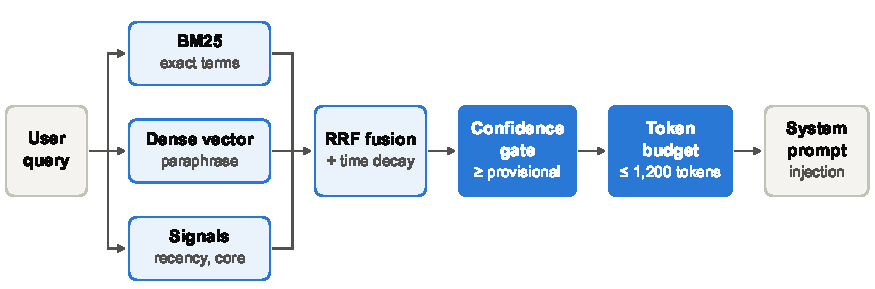
\includegraphics[width=0.85\linewidth]{fig2_pipeline.pdf}
  \caption{Retrieval and injection pipeline. Dense and BM25 rankings fuse via
  RRF (BM25 from 300 thoughts); recency and core-fact thoughts are appended; a
  confidence gate removes non-injectable thoughts; a token budget caps
  injected context.}
  \label{fig:pipeline}
\end{figure}

% ══════════════════════════════════════════════════════════════════════════════
\section{Evaluation Setup}
\label{sec:setup}

I evaluate four research questions:

\begin{itemize}
  \item \textbf{RQ1}: Does memory injection raise the keyword-hit rate on
  personal questions?
        (A/B, end-to-end, \S\ref{sec:ab})
  \item \textbf{RQ2}: Which components contribute? (ablation,
        retrieval-layer, \S\ref{sec:ablation})
  \item \textbf{RQ3}: How do cost and ranking scale with memory size?
        (\S\ref{sec:scale})
  \item \textbf{RQ4}: Does cross-tool sharing work? (\S\ref{sec:crosstool})
\end{itemize}

{\sloppy
\paragraph{Models.} Gemini Flash-Lite (cloud; \texttt{gemini-flash-}\allowbreak\texttt{lite-latest},
queried 30 June 2026), gemma3:4b and qwen2.5:3b (local via Ollama). Answers used a 150-token limit and default sampling, one per
question and condition; the Gemini alias and Ollama tags are mutable, and local model digests were not recorded.\par}

\paragraph{A/B design.} Each of 30 synthetic English profiles consists of 5
build statements (identity, preferences, positions, decisions) followed by 5
test questions with a known expected keyword. Each statement is made once and
firmly (``I prefer\ldots''), which is enough to reach provisional
(\S\ref{sec:lifecycle}). Each question is answered \emph{with memory} (through
the Noesis proxy) and \emph{without} (direct to the provider); all models get
the identical first $110$ questions (22 profiles). An answer counts as a hit
if it contains the expected keyword, and I report the keyword-hit rate; paired
outcomes are tested with McNemar's $\chi^2$~\citep{mcnemar1947}.

\paragraph{Retrieval-layer experiments.} Ablation, scale, and cross-tool
experiments call the real pipeline's Python API without LLM calls, measuring
Recall@5, MRR, the recall and size of the injected context, tentative leakage,
and injected tokens; the cross-tool experiment simulates tools by labeling
each statement's source.

\paragraph{Integration routes.} Only the proxy, which injects context and
stores each exchange automatically, is evaluated end to end (\S\ref{sec:ab}).
MCP tools are model-controlled~\citep{mcpspec}: nothing is stored or injected
unless the model calls \texttt{remember} or \texttt{recall}, so timely use is
not ensured, and the MCP server has unit tests only. The browser extension
only captures turns and is not evaluated.

\paragraph{Reproducibility.} A released script
(\texttt{experiments/verify\_paper.py}) recomputes every experimental number
in this paper from the raw result files and reads the lifecycle constants from
the source. The ablation and scale experiments were re-run in October 2026
with the June software (Python 3.12.11, torch 2.2.2, transformers 4.44.2,
sentence-transformers 3.0.1, all-MiniLM-L6-v2) and reproduced the June numbers
exactly before the metric corrections (\S\ref{sec:limitations}) and the top-5
baseline were added. The script audits arithmetic, not answer scoring, and the
saved records are incomplete: the local-model A/B runs kept the first 150
characters of each answer and the end-to-end run the first 100 (hits were
scored on full answers); the Gemini A/B records were recovered from the run's
console log, which printed only hit marks; and no run kept prompts or injected
contexts. Answers therefore cannot be re-scored from the released files. Code,
data, and paper sources are tagged \texttt{v1.0-preprint}.

% ══════════════════════════════════════════════════════════════════════════════
\section{Results}
\label{sec:results}

\subsection{RQ1: Memory injection raises the keyword-hit rate across model tiers}
\label{sec:ab}

\begin{table}[!htbp]
  \centering
  \caption{A/B keyword-hit rates on identical $n{=}110$ questions. All $p<0.001$
  (McNemar, df$=$1).}
  \label{tab:ab_results}
  \begin{tabular}{lccccc}
    \toprule
    \textbf{Model} & $n$ & \textbf{With} & \textbf{Without} & $\Delta$pp & $\chi^2$ \\
    \midrule
    Gemini Flash-Lite & 110 & 85.5\% & 41.8\% & \textbf{+43.6} & 42.48 \\
    gemma3:4b         & 110 & 82.7\% & 34.5\% & \textbf{+48.2} & 51.02 \\
    qwen2.5:3b        & 110 & 62.7\% & 37.3\% & \textbf{+25.5} & 16.57 \\
    \bottomrule
  \end{tabular}
\end{table}

\begin{figure}[!htbp]
  \centering
  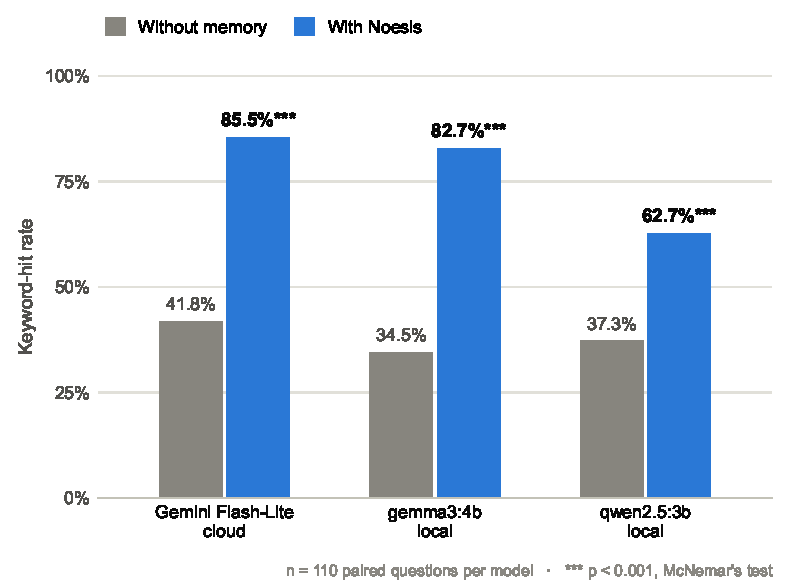
\includegraphics[width=0.78\linewidth]{fig3_ab_comparison.pdf}
  \caption{A/B keyword-hit rate across models ($n{=}110$ each). All improvements
  significant at $p<0.001$.}
  \label{fig:ab}
\end{figure}

Table~\ref{tab:ab_results} and Figure~\ref{fig:ab} show the headline result.
First, \emph{injection helps everywhere}: all three models improve
significantly, and memory \emph{hurt} in only 10 of 330 paired answers
(3.0\%). Because a profile's five questions share one memory store, I also
resampled whole profiles (20{,}000 draws over 22 profiles): the 95\% intervals
for the gains are $+34.5$ to $+51.8$pp (Gemini Flash-Lite), $+37.3$ to
$+59.1$pp (gemma3:4b), and $+13.6$ to $+36.4$pp (qwen2.5:3b), all above zero.
Second, \emph{memory levels the field between local and cloud}: with
injection, gemma3:4b reaches 82.7\%, close to Gemini Flash-Lite's 85.5\%, from
a lower baseline (34.5\% vs.\ 41.8\%). Third, \emph{the smallest model gains
least}: qwen2.5:3b reaches only 62.7\%; a model-capability ceiling is one
possible reason, but the saved runs do not record the injected context, so it
remains a hypothesis.

The hit rate alone does not separate retrieval strategies at this scale. In a
separate end-to-end run (50 questions, 10 profiles, Gemini Flash-Lite),
Noesis, injecting every stored memory, and injecting the five most recent
scored 41, 40, and 41 of 50, against 22 with no memory; with only 3--9
memories per profile, all three inject nearly the same context. The A/B result
therefore shows that personal context helps on these tasks, not that the
lifecycle beats simpler ways of supplying the same memories.

\subsection{RQ2: Semantic retrieval drives recall; gating keeps tentative thoughts out}
\label{sec:ablation}

\begin{table}[!htbp]
  \centering
  \caption{Ablation and baselines (50 queries over 28 memories, 5 tentative;
  retrieval-layer, 2{,}000-token budget). A retrieved memory counts only if it
  is the ground-truth memory. Recall@5 and MRR use the first five memories in
  injection order (or all, if fewer are returned); context recall, items, and
  leak cover everything injected, and leak counts tentative memories among those
  slots.}
  \label{tab:ablation}
  \begin{tabular}{lccccc}
    \toprule
    \textbf{Config} & \textbf{Recall@5} & \textbf{MRR} & \textbf{Context recall} & \textbf{Items} & \textbf{Leak} \\
    \midrule
    \textbf{Noesis (full)}   & \textbf{99\%} & \textbf{1.000} & \textbf{100\%} & \textbf{10.9} & \textbf{0/546} \\
    w/o core-fact signal     & 99\% & 1.000 & 100\% & 9.7  & 0/487 \\
    w/o recency signal       & 99\% & 1.000 & 100\% & 9.7  & 0/484 \\
    w/o confidence gating    & 99\% & 1.000 & 100\% & 11.5 & \textbf{73/573} \\
    w/o semantic retrieval   & 24\% & 0.105 & 24\%  & 5.0  & 0/250 \\
    \midrule
    Top-5 RAG                & 99\% & 1.000 & 99\%  & 5.0  & 19/250 \\
    Recent-window            & 17\% & 0.084 & 17\%  & 5.0  & 50/250 \\
    Random                   & 12\% & 0.063 & 12\%  & 5.0  & 51/250 \\
    \bottomrule
  \end{tabular}
\end{table}

Each Noesis variant runs the real context builder with one component switched
off; the baselines draw from every stored memory, tentative ones included.
Status and confidence are assigned when the test store is built, so the suite
tests whether retrieval respects those labels, not how the lifecycle derives
them. At 28 memories the semantic channel is dense retrieval alone, and
stale-memory leakage is measured only by the supersession test
(Table~\ref{tab:supersession}).

Removing semantic retrieval collapses recall (99\%$\to$24\%;
Table~\ref{tab:ablation}). Removing the confidence gate leaves recall
unchanged but lets tentative thoughts into 73 of 573 injected slots, where the
full system injects none. Ungated top-5 retrieval ranks as well as Noesis
(Recall@5 99\%, MRR 1.000), as it does at scale (\S\ref{sec:scale}), but lets
a tentative thought into 19 of its 250 slots. A separate poisoning test
agrees: with 5 settled facts and 8 hedged statements contradicting them,
ungated top-5 retrieval returned a hedged statement in 13 of 25 slots across 5
queries, and Noesis returned none. Both tests use hedged statements; a firmly
stated false one would pass the gate (\S\ref{sec:limitations}). Removing the
core-fact or recency signal does not change recall: each adds about one memory
per query (10.9 vs.\ 9.7 items), and because the builder appends them after
the eight semantic results, they never reach the first five slots. Whether
they help on queries that semantic retrieval misses needs a dedicated query
set.

\subsection{RQ3: Retrieval keeps cost flat as memory grows}
\label{sec:scale}

\begin{figure}[!htbp]
  \centering
  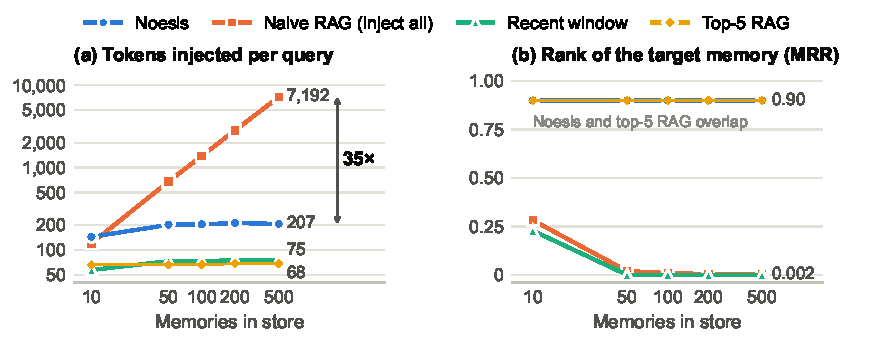
\includegraphics[width=0.88\linewidth]{fig4_scale_degradation.pdf}
  \caption{Scale behavior from 10 to 500 stored memories. (a) Noesis's
  injected tokens stay flat ($\sim$207) while naive RAG (inject all) grows to
  7{,}192 (35 times); top-5 RAG stays at 66--68. (b) Noesis and top-5 RAG
  hold MRR at 0.90; naive RAG collapses to 0.002
  as targets are buried; recent-window loses recall entirely past $n{=}10$.}
  \label{fig:scale}
\end{figure}

Figure~\ref{fig:scale} sweeps memory size from 10 to 500 with 10 known targets
embedded among fillers. Noesis's injected cost is flat (144$\to$207 tokens),
well under the 1{,}200-token budget, and MRR holds at 0.90: 9 of 10 targets
sit at rank 1 and the tenth is never retrieved. Naive RAG keeps recall only by
injecting everything: 7{,}192 tokens at $n{=}500$, with the target buried near
rank 500 (MRR 0.002). Recent-window recall collapses to 0\% beyond $n{=}10$. A
standard top-5 RAG (the query's five nearest memories) does as well: the same
9 of 10 targets at rank 1, with 66--68 tokens per query. Flat cost and good
ranking come from retrieval itself, not from anything specific to Noesis; what
Noesis adds is the gate (\S\ref{sec:ablation}). Recall alone is therefore
misleading; rank and token cost must be reported together.

\subsection{RQ4: Cross-tool sharing vs.\ structural isolation}
\label{sec:crosstool}

\begin{figure}[!htbp]
  \centering
  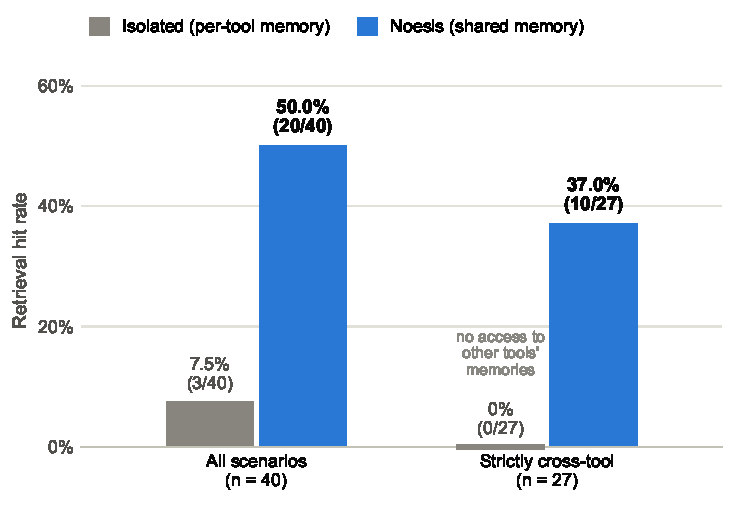
\includegraphics[width=0.7\linewidth]{fig6_cross_tool.pdf}
  \caption{Cross-tool retrieval. Isolated per-tool memory scores 0\% on
  strictly cross-tool queries by construction.}
  \label{fig:crosstool}
\end{figure}

Of 40 scenarios, 27 state a stance in one tool and ask about it from another;
in 7 the asking tool was one of two that stated it; in 6 a third tool asks
after two others did (Figure~\ref{fig:crosstool}). On the 27 strictly
cross-tool queries Noesis retrieves 37\% (10/27) and the isolated baseline
0\%, by construction, since the memory is not in its partition. Where the
asking tool did see the stance (7 scenarios), isolated memory retrieves 3 and
Noesis 6; over all 40, Noesis retrieves 50\% and the isolated baseline 7.5\%.
The comparison shows the value of access, not an advantage over another
shared-memory system given the same records. Noesis's misses trace to
retrieval precision (the memory exists but ranks below top-$k$), not to
sharing.

% ══════════════════════════════════════════════════════════════════════════════
\section{The Star Map Visualization}
\label{sec:viz}

\begin{figure}[!htbp]
  \centering
  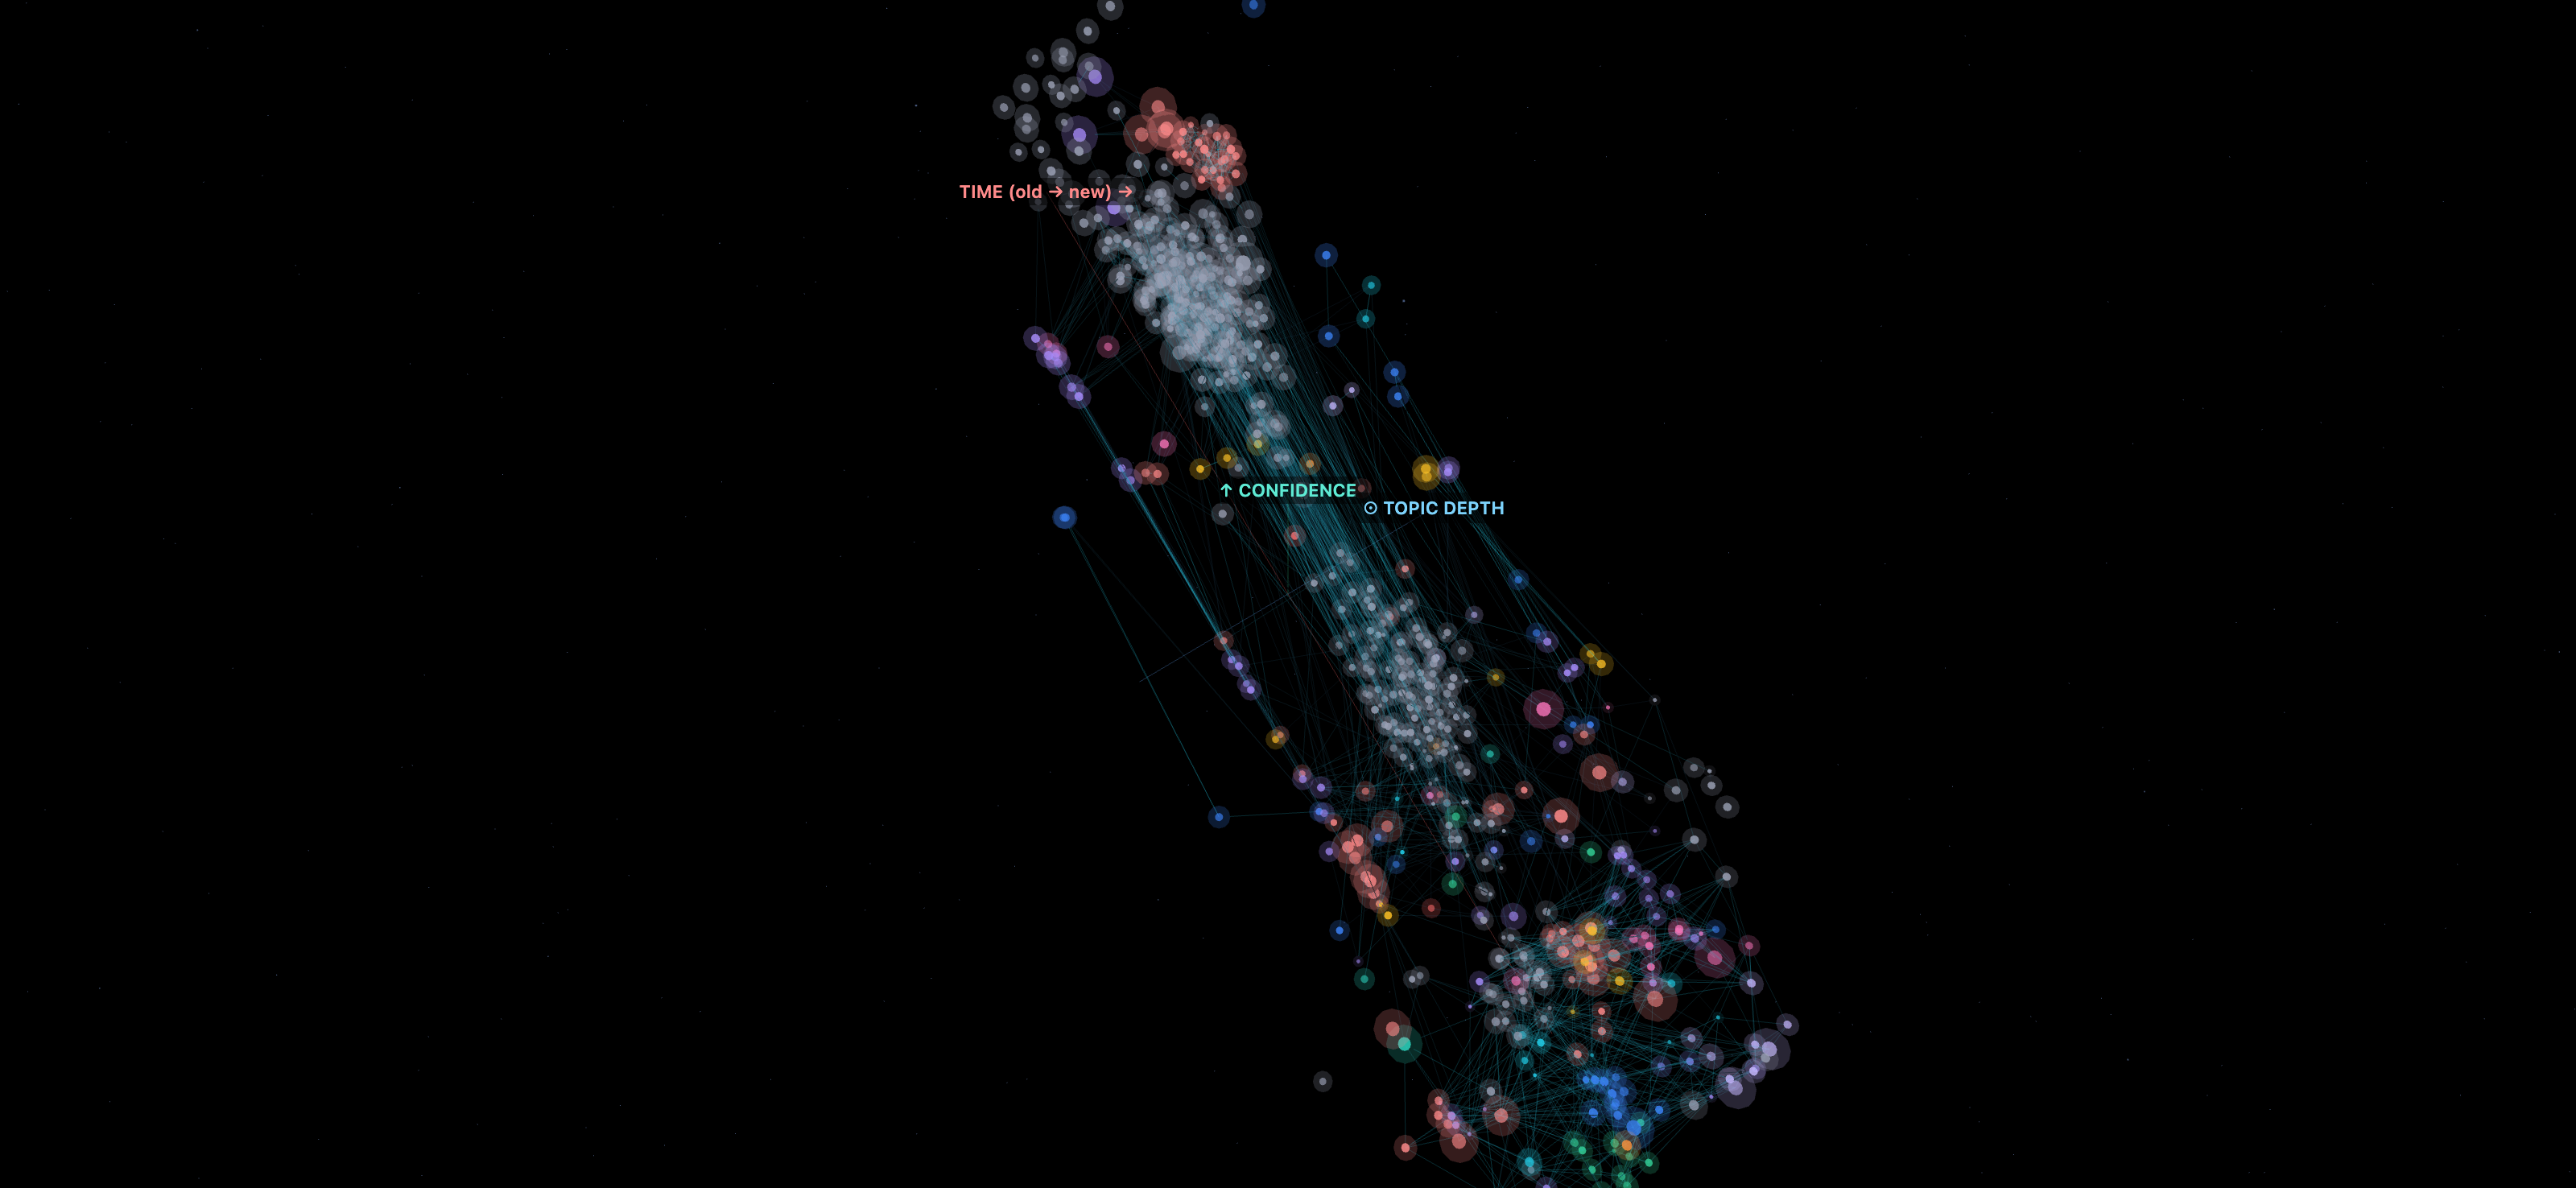
\includegraphics[width=0.85\linewidth]{fig5_star_map.png}
  \caption{The star map. Semantic neighbors cluster; time runs from older (left) to
  newer (right), height shows confidence, color shows topic, and size and
  brightness show type and activation weight.}
  \label{fig:starmap}
\end{figure}

The star map shows the stored thoughts as a galaxy (Figure~\ref{fig:starmap}),
placed by a short force simulation: weak springs pull each star toward its
creation time (horizontal) and confidence (vertical), semantic attraction
pulls it toward its most similar neighbors (cosine $\geq 0.45$), and repulsion
separates topics. Clusters therefore form from embedding similarity while time
and confidence stay readable, and hovering a star shows its text and
confidence. The store shown is the local development store, filled by
experiment and demo runs: of its 601 thoughts, 355 sit in the catch-all
``general'' topic and 18 have settled, which shows how coarse topic assignment
still is. The viewer opens the store read-only, and its edges never affect
retrieval, so the map says nothing about whether graph structure improves
answers.

% ══════════════════════════════════════════════════════════════════════════════
\section{Discussion}
\label{sec:discussion}

\paragraph{When memory helps most.} Gains concentrate on questions
unanswerable without personal context (job, stack, stances); on mainstream
questions both conditions often answer correctly. Other factors push the other
way (\S\ref{sec:limitations}), so these gains should not be read as an upper
or lower bound.

\paragraph{Memory can close the local--cloud gap.} gemma3:4b gains most
($+48.2$pp; $+139\%$ over its baseline) and approaches Gemini Flash-Lite with
memory, while qwen2.5:3b gains least ($+25.5$pp; \S\ref{sec:ab}), so the
benefit is not monotonic in model size. It is largest for small local models
that can use the injected context, which matters for private and offline use.

\paragraph{Retrieval precision is the current bottleneck.} The cross-tool
misses and several A/B misses are ranking failures: the memory is stored but
ranks below the cut, so better ranking (rerankers, query expansion) is the
highest-leverage next step. The supersession fix's residual 7\% is different:
in both leaks the detector never fired, because its lexicon lacked the
replacement verb in one case and the domain (Node.js) in the other.

\paragraph{Noesis inside an agent harness.} An execution harness manages a
task's control flow, tools, state, and recovery~\citep{anthropicharness};
Noesis would serve inside one as memory, not orchestration, though this is
neither implemented nor evaluated here. The harness would insert approved
memories for the current user, project, and scope as a bounded, sourced block
and send back candidate memories with their sources; Noesis could fill
LangGraph's cross-thread store, not its thread checkpoints~\citep{langgraph}.
Integration also needs corrections, deletion, audit, and source lineage, and
three gaps stand out: repetition counts similar records whatever their source,
and the proxy stores each request's full history, so replays and assistant
paraphrases can inflate confidence (unmeasured); new memories become
injectable only after asynchronous scoring; and injected memories are neither
marked as data nor deduplicated against the harness's summaries.

\paragraph{Graph structure.} The evaluated system is not a graph-based
reasoner. Supersession links are implemented and evaluated
(Table~\ref{tab:supersession}); topic clusters and wiki links are not
evaluated separately; and the one-hop expansion over vault links cannot add a
memory (it writes 8-character identifiers but looks up 12-character ones).
Every reported result comes from flat retrieval.

\paragraph{Negative results.} I report that the supersession check initially
never ran, so stale stances leaked 93\% of the time
(\S\ref{sec:supersession}); that core-fact and recency signals added no recall
in my ablation; that top-5 RAG matches Noesis's ranking at lower cost; that
the 3B model gains least; and that the graph expansion never adds a memory. I
consider these findings part of the contribution.

% ══════════════════════════════════════════════════════════════════════════════
\section{Future Work}
\label{sec:future}

\paragraph{Thought branching.} When a new judgment deviates from history by
more than a threshold ($\delta = 1-\cos > 0.45$), Noesis should branch via
\texttt{evolved\_from} rather than supersede, preserving a stance's trajectory
and enabling metrics such as stabilization depth and branching rate.

\paragraph{Structured injection.} Replacing flat context lines with a
structured \texttt{user\_thought\_graph} may help small models use injected
memory. Typed, timed claims with support, contradiction, derivation, and
supersession relations would let ``PostgreSQL for analytics'' and ``MySQL for
a legacy app'' coexist, as in Zep~\citep{zep}; derived claims are not
independent evidence, so graph centrality should not raise confidence, and the
deciding test crosses flat and graph-backed stores with and without the same
gate.

\paragraph{Stronger evaluation.} LLM-as-judge scoring to complement keyword
hits; distractor questions; a second cloud model; longitudinal data beyond
synthetic profiles; and a harness-level comparison of native harness memory, a
simple shared store, and Noesis, with model, tasks, tools, and budget fixed.
Questions about alternatives the user was considering need tentative thoughts,
so excluding them should be compared with retrieving them with their
uncertainty and source, adapting the risk--coverage view of selective
prediction~\citep{geifman2017selective}. Counting repetition only across
distinct user statements would close the first gap in \S\ref{sec:discussion}.

% ══════════════════════════════════════════════════════════════════════════════
\section{Limitations}
\label{sec:limitations}

Keyword-hit scoring checks whether an answer contains the expected keyword,
not whether it is right: ``you do not prefer Python'' contains the same
keyword as ``you prefer Python'', and a correct answer worded differently or
in another language counts as a miss. Personas are synthetic, build/test
alignment may overstate real gains, and real conversations are noisier. The
cloud A/B uses one provider and $n{=}110$ rather than the planned 150: rate
limits stopped the 30 June run after 111 questions, and I did not add the 35
answered in a later session because the
\texttt{gemini-flash-}\allowbreak\texttt{lite-latest} alias may by then have
pointed to another model. Retrieval-layer experiments measure what reaches the
prompt, not answer quality. The supersession detector relies on replacement
verbs and a domain keyword map, and its 93\%~$\to$~7\% result is in-sample: it
was developed on the same 30 scenarios, and held-out paraphrases, unseen
domains, and legitimate simultaneous preferences (which a domain match could
wrongly retire) are needed. On the scale benchmark top-5 RAG ties Noesis on
ranking. The ablation and poisoning leak counts were corrected in October 2026
to stop counting settled memories that merely shared a word with a tentative
one (for example, ``Kafka''). After an external review, I changed the ablation
in five ways: it scores exact memory identity instead of shared phrases such
as ``I prefer''; it drops ``Precision@5'', which measured non-tentative
results rather than relevant ones; it runs every variant through the same
context builder, so each differs from the full system in one component only;
it applies the memories' ages, which the test store had dropped; and it lets
the recent-window and random baselines return tentative memories. This lowered
the weak baselines (random 45\%~$\to$~12\%, w/o semantic 49\%~$\to$~24\%
Recall@5); Noesis moved from 100\% to 99\%. No result has been independently
replicated.

Noesis also adds an attack surface: the local proxy sees every request,
including provider API keys and full conversations; optional cloud extraction
sends conversation text to a third party; and because one firmly stated
sentence reaches provisional (\S\ref{sec:lifecycle}), a planted or mistaken
statement can enter future prompts. The gate filters hedged statements but is
no defense against deliberate poisoning.

% ══════════════════════════════════════════════════════════════════════════════
\section{Conclusion}
\label{sec:conclusion}

Injecting a user's own memories raised all three models' keyword-hit rates on
personal questions, though whether Noesis's lifecycle beats simpler ways of
supplying them is not yet shown. Its gate kept tentative and hedged statements
out of the prompt in constructed tests where plain retrieval let them in.
Retrieval keeps cost flat (35 times cheaper than injecting everything at
$n{=}500$; top-5 RAG is cheaper still), and a shared per-user store gives
every tool the same records. The result is a local-first layer that brings a
4B local model's keyword-hit rate close to a small cloud model's (82.7\% vs.\
85.5\%; the gap is not significant, though that does not make them equal) and
keeps the user's reasoning in the user's own vault.

\section*{Acknowledgments}
AI coding assistants were used in this work. ZCode (Z.ai, GLM models)
assisted with implementing the experiment scripts and drafting the original
experiment reports. Claude (Anthropic) was used to review the manuscript,
revise its text, redesign the figures, write the verification script
(\texttt{experiments/verify\_paper.py}), and re-run the retrieval-layer
experiments in October 2026. All reported numbers are checked against the
raw results by that script, and the author takes full responsibility for the
paper's content.

% ══════════════════════════════════════════════════════════════════════════════
\begin{multicols}{2}
\bibliographystyle{plainnat}
\bibliography{references}
\end{multicols}

\end{document}
